\documentclass{beamer}
%
% Choose how your presentation looks.
%
% For more themes, color themes and font themes, see:
% http://deic.uab.es/~iblanes/beamer_gallery/index_by_theme.html
%
\mode<presentation>
{
  \usetheme{Boadilla}      % or try Darmstadt, Madrid, Warsaw, ...
  \usecolortheme{default} % or try albatross, beaver, crane, ...
  \usefonttheme{default}  % or try serif, structurebold, ...
  \setbeamertemplate{navigation symbols}
} 

\usepackage[english]{babel}
\usepackage[utf8x]{inputenc}
\usepackage{pdfpages}
\usepackage{float}

\newenvironment<>{varblock}[2][.9\textwidth]{%
  \setlength{\textwidth}{#1}
  \begin{actionenv}#3%
    \def\insertblocktitle{#2}%
    \par%
    \usebeamertemplate{block begin}}
  {\par%
    \usebeamertemplate{block end}%
  \end{actionenv}}

\title[Neuroanatomy workshop 3]{The Sensory-motor System}
\author{JJ Torre}
\institute{Parietal Team - INRIA Saclay}
\date{2018}

\begin{document}

\begin{frame}
  \titlepage
\end{frame}

% Uncomment these lines for an automatically generated outline.
%\begin{frame}{Outline}
%  \tableofcontents
%\end{frame}

\section{Introduction}

\begin{frame}{Introduction}
 \begin{columns}[T]
  \begin{column}{.4\textwidth}
    \begin{itemize}
      \item The sensory-motor system constitutes our main means of receiving input (sensory
      stimuli) and producing output (movement) in relation to the environment
      \item It follows a hierarchical organization common to both motor and sensory systems
    \end{itemize}

    \vspace{-.3cm}
    \begin{varblock}[5cm]{\scriptsize Peripheral Nervous System (PNS)}
     \scriptsize Although we are going to focus on the central nervous system, a lot is going on before reaching the brain! Motor reflexes happen at this level
    \end{varblock}
  \end{column}
  \begin{column}{.6\textwidth}
   \begin{figure}[H]
   \vspace*{-1.25cm}
    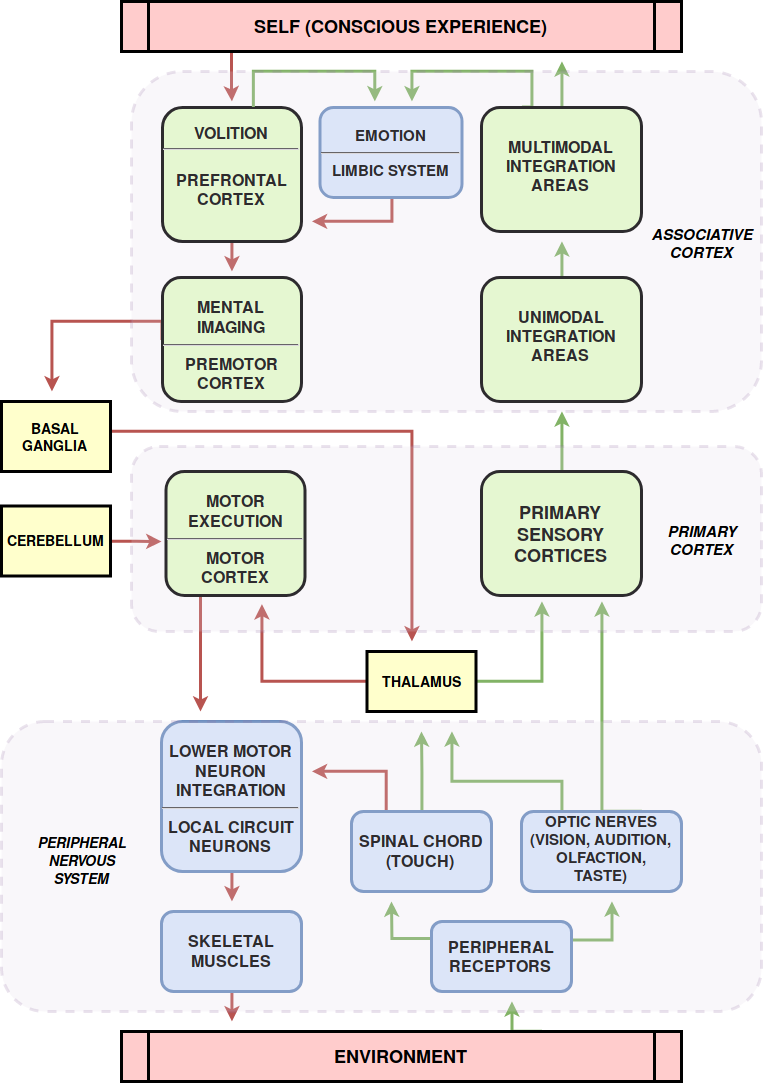
\includegraphics[width=.85\textwidth]{figures/brain_and_env.png}
   \end{figure}
  \end{column}
 \end{columns}
\end{frame}

\begin{frame}{Primary Areas}
    \begin{columns}[T]
  \begin{column}{.4\textwidth}
    \begin{itemize}
      \item \small Primary areas receive input directly from the thalamus
      \item \small Sensory areas receive high-dimensional data for each modality (vision, audition, etc.)
      \item \small The motor cortex conveys the already planned movement and sends it to the muscles
      \item \small Primary cortices have the better and most differentiated 6-layer laminar structure
    \end{itemize}
  \end{column}
  \begin{column}{.6\textwidth}
   \begin{figure}[H]
    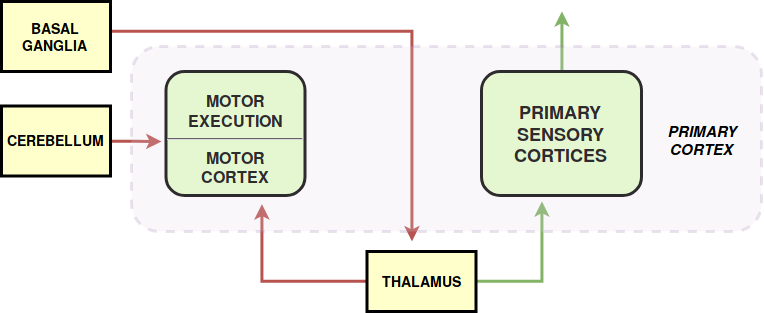
\includegraphics[width=1\textwidth, height=3.5cm]{figures/primary_structures.png}
   \end{figure}
   \vskip
   \begin{varblock}[7cm]{\scriptsize Olfaction is a special boy}
    \scriptsize Olfaction is the only sense that does not do thalamic relay in its
    path to the cortex. Signals from the nose go directly to the piriform cortex via the
    olfactory tract.
   \end{varblock}
  \end{column}
 \end{columns}
\end{frame}



\section{Some \LaTeX{} Examples}

\subsection{Tables and Figures}

\begin{frame}{Tables and Figures}

\begin{itemize}
\item Use \texttt{tabular} for basic tables --- see Table~\ref{tab:widgets}, for example.
\item You can upload a figure (JPEG, PNG or PDF) using the files menu. 
\item To include it in your document, use the \texttt{includegraphics} command (see the comment below in the source code).
\end{itemize}

% Commands to include a figure:
%\begin{figure}
%\includegraphics[width=\textwidth]{your-figure's-file-name}
%\caption{\label{fig:your-figure}Caption goes here.}
%\end{figure}

\begin{table}
\centering
\begin{tabular}{l|r}
Item & Quantity \\\hline
Widgets & 42 \\
Gadgets & 13
\end{tabular}
\caption{\label{tab:widgets}An example table.}
\end{table}

\end{frame}

\subsection{Mathematics}

\begin{frame}{Readable Mathematics}

Let $X_1, X_2, \ldots, X_n$ be a sequence of independent and identically distributed random variables with $\text{E}[X_i] = \mu$ and $\text{Var}[X_i] = \sigma^2 < \infty$, and let
$$S_n = \frac{X_1 + X_2 + \cdots + X_n}{n}
      = \frac{1}{n}\sum_{i}^{n} X_i$$
denote their mean. Then as $n$ approaches infinity, the random variables $\sqrt{n}(S_n - \mu)$ converge in distribution to a normal $\mathcal{N}(0, \sigma^2)$.

\end{frame}

\end{document}
